\documentclass[letterpaper,10pt]{article}
\usepackage[utf8]{inputenc}
\usepackage[top=1in, bottom=1in, left=1in, right=1in]{geometry}
\usepackage{parskip}
\usepackage{tabularx}
\usepackage{qtree}
\usepackage{graphicx}
\usepackage{xfrac}
\usepackage{forest}
\usepackage{tikz-dependency}
\usepackage{graphicx}
\usepackage{float}
\usepackage{amsmath}
\usepackage{varioref}
\usepackage{hyperref}
\usepackage{xfrac}
\usepackage{amsmath}
\usepackage{bm}
\usepackage{pgfplots}
\usepackage{pbox}
\usepackage{framed}
\usepackage{titlesec}
\usepackage[authordate,bibencoding=auto,strict,backend=biber,natbib]{biblatex-chicago}
\usepackage{enumitem}
\renewcommand{\cite}{\citep}

%\newcommand{\sectionbreak}{\clearpage}

\DeclareMathOperator*{\argmin}{arg\,min}
\DeclareMathOperator*{\argmax}{arg\,max}

\addbibresource{prop.bib}

%opening
\title{Incrementally Identifying Objects from Referring Expressions using Spatial Object Models}
\author{Gaurav Manek}

\begin{document}

\maketitle


\section{Research Question}

We want to parse referring expressions incrementally,  identifying objects in physical scenes.

We assume that we have access to:
\begin{enumerate}[topsep=0pt,itemsep=-1ex,partopsep=1ex,parsep=1ex]
 \item an object model that includes the position of each object, and
 \item a language model that, when provided with a noun phrase, can return a probability distribution over objects that it may refer to.
\end{enumerate}

We use this information to construct an incremental parser that takes referring expressions as input and produces a probability distribution of possible objects that the expression is identifying.

(This thesis project will build on work done from Fall 2014 to present. Some work was previously completed in collaboration with undergraduate student Zachary Loery.)

\section{Significance}

Incremental parsing of referring expressions is an important problem because referring expressions are commonly used in natural human language when identifying objects. Improving on the ability of a robot to understand these expressions and making this understanding incremental can facilitate more natural human-robot interaction, especially in tasks where the robot needs to identify one object from many.

Currently, referring expression parsing is done with the entire referring expression as input: the $G^3$ framework by \citet{tellex2011understanding}, work done by \citet{UW_RSE_ICML2012}, and the parser developed by \citet{artzi2013weakly}, all require a complete sentence. Since the robot is presented with the input one word at a time, batch mode requires waiting for the complete utterance before processing and providing output, which takes time to complete. For example, practical implementations of the $G^3$ system can take up to 30 seconds from the end of the input and the start of a response. 

Our incremental parsing updates the distribution with each added word, substantially reducing the delay between input and response.

Incremental parsing also allows the robot to provide social feedback to the human. The robot could, for example, transition from a confused to a smiling face as more input words reduce the uncertainty of the referring expression.

Referring expression parsing is also closely related to the common robot task of pick-and-place, and could thus be a useful improvement for the Baxter robot and the H2R lab. 


\subsection{Examples}
Given a \textit{red apple}, \textit{blue tape}, \textit{red bowl}, and a \textit{metal bowl} scattered on a table, we want to be able to convert referring expressions similar to these into probability distributions over the objects:
\begin{enumerate}[topsep=0pt,itemsep=-1ex,partopsep=1ex,parsep=1ex]
 \item ``The object between the apple and the tape.''
 \item ``The red object.''
 \item ``The red thing on the left of the bowl.''
 \item ``The red thing on the left.''
 \item ``The thing on the left of the bowl.''
\end{enumerate}
Parsing a referring expression and finding a distribution over possible objects has been accomplished by \citet{tellex2011understanding},\citet{UW_RSE_ICML2012}, and \citet{artzi2013weakly}, among others.

\begin{figure}[h!tb]
  \centering
    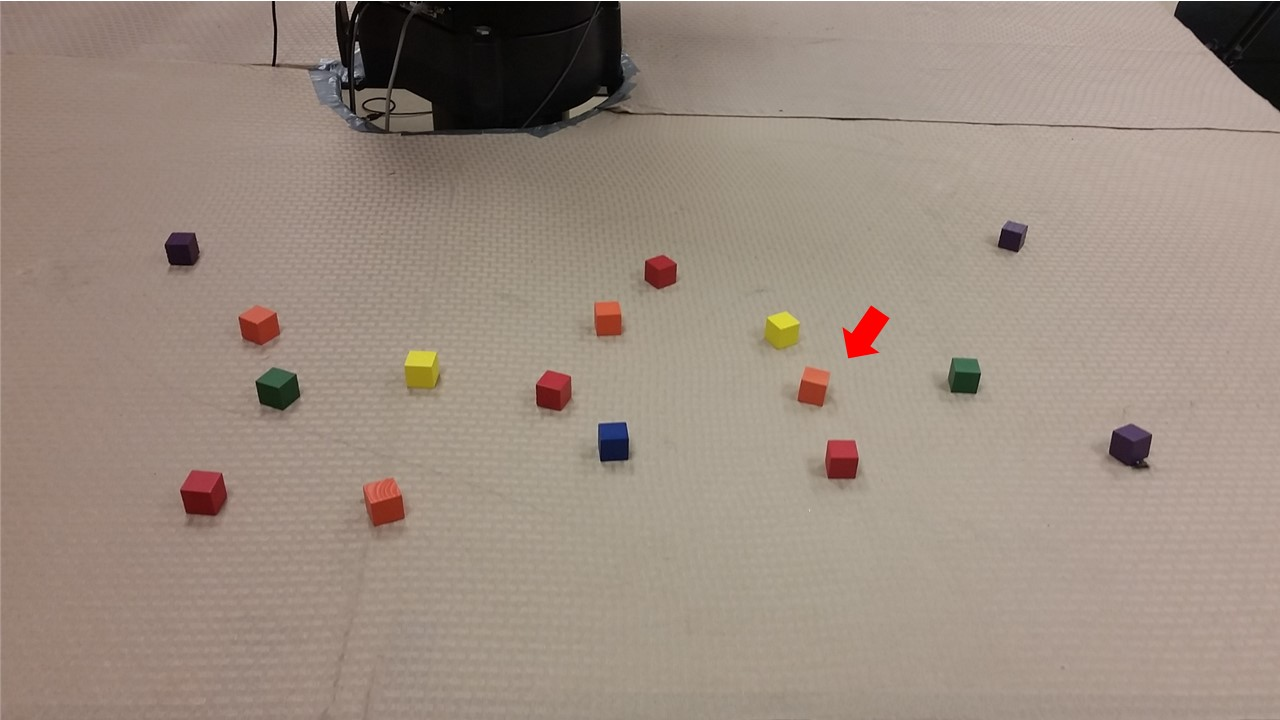
\includegraphics[width=0.66\textwidth]{worked_example_scene}
  \caption{Arrangement of objects on a table.}
  \label{fig:worked_example_table}
\end{figure}

We want to be able to parse these referring expressions incrementally, including each new word in our understanding of the referring expression as we receive it. Given the referring expression ``The orange cube between the red and the yellow'' to refer to the indicated object in 
Figure~\ref{fig:worked_example_table}, our model should give better estimations of the correct object as we receive more words in the referring expression:
\begin{enumerate}[topsep=0pt,itemsep=-1ex,partopsep=1ex,parsep=1ex]
\item ``The \ldots ''
\item ``The orange cube \ldots ''
\item ``The orange cube between the red and \ldots ''
\item ``The orange cube between the red and the yellow.''
\end{enumerate}
Figure~\ref{fig:worked_example_incremental} shows how the distribution over all objects changes with more words of the referring expression.

\begin{figure}[h!tb]
  \centering

\newcommand{\dist}[8]{\begin{tikzpicture}[trim axis left]
\begin{axis}[
	width=1.2in,
	height=0.6in,
	scale only axis,
	xticklabel=\empty,
	xtick=\empty,
	ytick=\empty,
	xlabel=Object,
	x label style={yshift=10pt},
	y label style={yshift=-24pt},
	ybar interval=0.9,
	enlarge x limits=-0.3,
	ymax=1.1, ymin=0.0,
	xmin=1, xmax=9,
]
\addplot 
	coordinates {(1,#1) (2,#2)
		 (3,#3) (4,#4) (5,#5) (6,#6) (7,#7) (8,#8) (9,0) };
\end{axis}
\end{tikzpicture}}

\begin{tabular}{cccc}
\dist{0.1}{0.1}{0.1}{0.1}{0.1}{0.1}{0.1}{0.1} & \dist{0.2}{0.01}{0.2}{0.2}{0.01}{0.01}{0.2}{0.01} &\dist{0.3}{0.01}{0.3}{0.1}{0.01}{0.01}{0.3}{0.01} & \dist{0.05}{0.}{0.8}{0.05}{0.}{0.}{0.05}{0.} \\
\textit{``The\ldots} &
\textit{\ldots orange cube\ldots} &
\textit{\ldots between the red\ldots} &
\textit{\ldots and the yellow.''} \\
\end{tabular}
  \caption{Probability distribution over all objects for incremental parts of ``The orange cube between the red and the yellow.''}
  \label{fig:worked_example_incremental}
\end{figure}


\section{Technical Approach}

Here we describe the general approach of our algorithm, how we parse referring expressions, and how we plan on making parsing both efficient and incremental.

We represent the referring expression as a tree, updating it each time we receive a new token. This representation allows us to perform computationally-intensive tasks once and cache intermediate results. This strategy allows us to produce intermediate results without having to recompute the entire expression so far.

More precisely, we construct a semantic tree such that each leaf node in the tree refers to some object. This tree is constructed by tagging the input using conditional random fields and then using deterministic transformations to turn that into a tree. We convert each of the leaf nodes into distributions over objects using a language model, and then finally evaluate this structure to obtain the final distribution. Here is a concrete example: 

We attempt to locate the \textit{orange cube} using the following referring expression: ``The orange cube between the red thing and the yellow thing.'' A selection of \textit{red}, \textit{blue}, \textit{orange}, \textit{purple}, \textit{green}, and  \textit{yellow} cubes are arranged on a table, as shown in Figure~\ref{fig:worked_example_table}. The orange cube referred to in the above statement is pointed to by a red arrow in the figure. The process of estimating the object from this information is:

\renewcommand{\tabularxcolumn}[1]{>{\small}m{#1}}
\begin{tabularx}{\textwidth}{@{} >{\hsize=.5\hsize \centering}X >{\hsize=.45\hsize}X @{}} 
\multicolumn{2}{c}{``The orange cube between the red thing and the yellow thing.''} \\ 
\multicolumn{2}{c}{$\Downarrow$} \\ 
% Chunking	
$\underbrace{\text{The orange cube}}_{\texttt{SNP}}$
$\underbrace{\text{between}}_{\texttt{PRP}}$
$\underbrace{\text{the red thing}}_{\texttt{SNP}}$
$\underbrace{\text{and}}_{\texttt{PRP}}$
$\underbrace{\text{the yellow thing}}_{\texttt{SNP}}$
$\underbrace{\text{.}}_{\texttt{.}}$
& 
\textbf{Tagging}

First, we use Mallet, \citep{McCallumMALLET} a sequence tagging library, to tag the referring expression with a set of tags.

The grammar is a subset of English grammar, and is developed to suit our use case.
\\ $\Downarrow$ \\[0.2cm] 

\scalebox{.9}{\Tree [.TARGET \qroof{The orange cube}.OBJECT [.BETWEEN   \qroof{the red thing}.OBJECT \qroof{the yellow thing}.OBJECT ] ]} &

\textbf{Semantic Tree}

The tagged sequence is then converted to a semantic tree. Because of the simplified tag set in the previous step, this transformation is simple.

\\ $\Downarrow$ \\[0.2cm] 

\scalebox{.9}{\Tree [.TARGET \qroof{$\{\sfrac{1}{16}, \sfrac{1}{16}, \cdots \sfrac{1}{16}\}$}.OBJECT [.BETWEEN   \qroof{$\{0, \sfrac{1}{8}, \cdots 0\}$}.OBJECT \qroof{$\{0, 0, \cdots, \sfrac{1}{2}\}$}.OBJECT ] ]} 

~

\scriptsize{\{\textit{orange\_1}, \textit{red\_1}, $\cdots $ \textit{yellow\_2}\}}

&
\textbf{Language Model}

We use a language model to convert each of the simple noun phrases into individual distributions over possible objects.

\\ $\Downarrow$ & ~ \\[0.2cm] 

\scalebox{.9}{\Tree [.TARGET \qroof{$\{90\%, 2\%, \cdots 1\%\}$}.OBJECT ]} 

~

\scriptsize{\{\textit{orange\_1}, \textit{orange\_2}, $\cdots $ \textit{blue\_1}\} }

&
\textbf{Bottom-up Evaluation}

We evaluate the tree bottom-up, using spatial features and trained weights to convert each input distribution and the type of preposition into a set of output scores. The final result is the object with the highest score.
\end{tabularx}

% \subsection{Mathematical Models}
% We have already devised mathematical models to evaluate referring expressions in batch mode. One of the tasks in this project is to factor these models for incremental use.

\subsection{Tagging and Semantic Tree construction}

We model the relationship between words and tags as a conditional random field, where the tag for any particular word depends on the neighboring words. We directly estimate the distribution of tags using the existing library Mallet, developed by \citet{McCallumMALLET}.

The transformation from the tagged sequence to the semantic tree is entirely deterministic, as the tags are tailored to the specific form of the queries in the corpus.

\subsection{Language Model for Objects}

The language model used is unigram language model, where each word $w_i$ refers to object $o_j$ with some joint score $Q(O = o_j, W = w_i)$ that we can estimate statistically. 
The distribution of simple noun phrase $S = (w_0, w_1, \cdots w_k)$ referring to object $o_j$ is, therefore:

\begin{align*}
	\Pr(O = o_i | S = (w_0, w_1, \cdots)) & = \frac{\Pr(O = o_i \cap S = (w_0, w_1, \cdots ))}{\Pr(S = (w_0, w_1, \cdots))}
\\ & \propto \Pr(O = o_i \cap S = (w_0, w_1, \cdots))
\\ & \approx \prod_{w_i \in (w_0, w_1, \cdots)} \left( (1 - \alpha) * \frac{Q(O = o_j, W = W_i)}{\sum_{o} Q(O = o, W = w_i)} + \alpha * \frac{1}{k} \right)
\end{align*}

For smoothing, we assume that there is some small probability $\alpha$ that the object is uniformly at random chosen without regard to the word. We arbitrarily set $\alpha \approx 5\%$.

\subsection{Bottom-up Evaluation}

Once we have a semantic tree, we can recursively simplify the tree to obtain the final distribution. Figure~\ref{fig:bottom_up_eval} illustrates this process and the two possible cases we apply to convert the tree into a distribution over objects.

\begin{figure}[h!tb]
  \centering
\begin{tabular}{ccccccc}
\Tree [.$\vdots$ \emph{The orange cube} [.{\emph{between}} \emph{the red} \emph{the yellow} ]] &
\pbox{0.2in}{\vspace{0.5in}
$\Rightarrow$} &
\Tree [.$\vdots$ $X_1$ [.{Preposition $p \in P$} $X_2$ $X_3$ ]] &
\pbox{0.2in}{\vspace{0.5in}
$\Rightarrow$} &
\Tree [.{$\vdots$} $X_1$ $T_1$ ]
&
\pbox{0.2in}{\vspace{0.5in}
$\Rightarrow$} & 
\Tree [.{$\vdots$} $T_0$ ]
\\ 
& & \textbf{(Case 1)} & & \textbf{(Case 2)}
\end{tabular}
\caption{The two cases of bottom-up evaluation.}
  \label{fig:bottom_up_eval}
\end{figure}

\textbf{Case 1}: Simplifying a preposition and associated noun-phrases.

We have preposition $p \in P = $ \{near, left, right, front, behind, between\}. Each grounding that the preposition relies on is modeled by the distributions $X_1, X_2, \cdots X_n$, obtained from the language model. $T$ is the distribution of the object that the user is referring to.

In Figure~\ref{fig:bottom_up_eval}, we illustrate how we simplify preposition $p$ with groundings $X_1$ and $X_2$ into a single distribution $T_1$.

We find $T$ with:
\begin{align*}
\Pr(T = o) & = \Pr(T = o | X_1, X_2, \cdots X_n, P = p)
\intertext{Assume that each grounding is independent and factor the expression:}
& = \sum_{o_1, o_2, \cdots o_n \in O} \Pr(T = o \cap P = p \cap X_1 = o_1, X_2 = o_2, \cdots X_n = o_n)
\\ & = \sum_{o_1, o_2, \cdots o_n \in O} \Pr(T = o \cap P = p | X_1 = o_1, X_2 = o_2, \cdots X_n = o_n) \cdot \Pr(X_1 = o_1, X_2 = o_2, \cdots X_n = o_n)
\intertext{Parametrize the probability with feature-vector function $f$, weights $\theta_p$, logistic function $S$, and some normalization factor $z$:}
& = \sum_{o_1, o_2, \cdots o_n \in O} \text{S}\left( \frac{f(o_1, o_2, \cdots, o_n) \cdot \theta_p}{z} \right) \cdot \prod_{i = 1}^n \Pr(X_i = o_i)
\end{align*}

We can estimate $\theta_p$ for each $p$ using logistic regression, and select feature-vector function $f$ separately.

\textbf{Case 2}: Combining multiple distributions.

In Figure~\ref{fig:bottom_up_eval}, we illustrate how we simplify groundings $X_1$ and independently derived distribution $T_1$ to get $T_0$, our estimated distribution.

In cases where we have multiple distributions, we estimate the true distribution by assuming each of $X_1, X_2, \cdots X_n$ are independent and taking the joint probability:
\begin{align*}
\Pr(T = o) & = \Pr(T = o | X_1, X_2, \cdots X_n)
\\ & = \Pr(X_1 = o, X_2 = o, \cdots X_n = o)
\\ & = \prod_{i = 1}^n\Pr(X_i = o)
\end{align*}
(We also assume that the prior distribution of $T$ is uniform over all objects.)

These two cases are sufficient to recursively reduce the tree into a single distribution.

\subsection{Incremental Parsing}

Incremental parsing will be achieved by using dynamic programming approaches to caching the current estimates of various nodes in the tree, and refining them based on new input. 

\section{Data Collection} 

Training each model that we use requires a lot of data. We collect many examples to train and test our system on as well as run our test set against humans to benchmark the performance of our system against.

We have collected a corpus of human-generated data using Human Intelligence Tasks (HITs) on the Amazon Mechanical Turk platform and hand-generated scenes. We additionally use AMT to have humans evaluate our test set to obtain a baseline.

\subsection{Referring Expression Generation}
A set of HITs were created to elicit referring expressions. A total of 19 scenes were constructed, each with a set of about 12 to 15 objects scattered on a table and at least 6 identical orange cubes. For each orange cube in each scene, 9 different workers were told to ask a robot across the table for the indicated orange cube. Figure~\ref{fig:ref_expr_elicit_pic} provides an example of such a labeled scene.

\begin{figure}[htb]
  \centering
    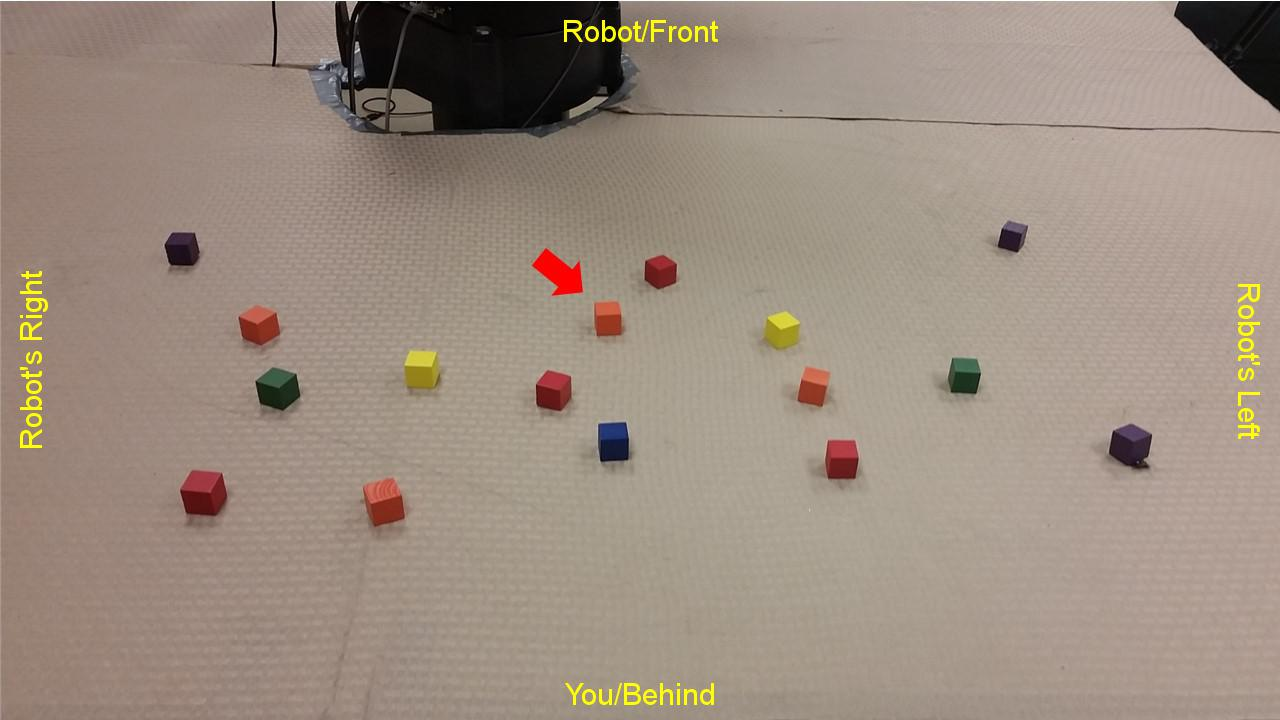
\includegraphics[width=0.75\textwidth]{ref_expr_elicit_pic}
  \caption{Example picture provided to HIT workers to elicit referring expressions.}
  \label{fig:ref_expr_elicit_pic}
\end{figure}

We provide the following instructions to respondents:

\begin{framed}
You are standing across the table from a robot. Write down what you would say to the robot if you wanted the indicated orange cube on the table.
\begin{itemize}[topsep=0pt,itemsep=-1ex,partopsep=1ex,parsep=1ex]
\item Use phrases like "between", "near", "left of", "right of", "in front of" and "behind".
\item Use front/behind/left/right from the robot's perspective, as labeled in the image. 
\item All orange cubes look the same.
\item You must ask for the item indicated by the red arrow
\item The instruction must be a single sentence.
\item Answer both questions.
\end{itemize}
\end{framed}

\subsection{Referring Expression Evaluation}

For each referring expression in the test set, we get three separate raters to identify the target and provide feedback on the ease of understanding of the referring expression. Figure~\ref{fig:ref_expr_eval_pic} shows an example scene.

\begin{figure}[h!tb]
  \centering
    \fbox{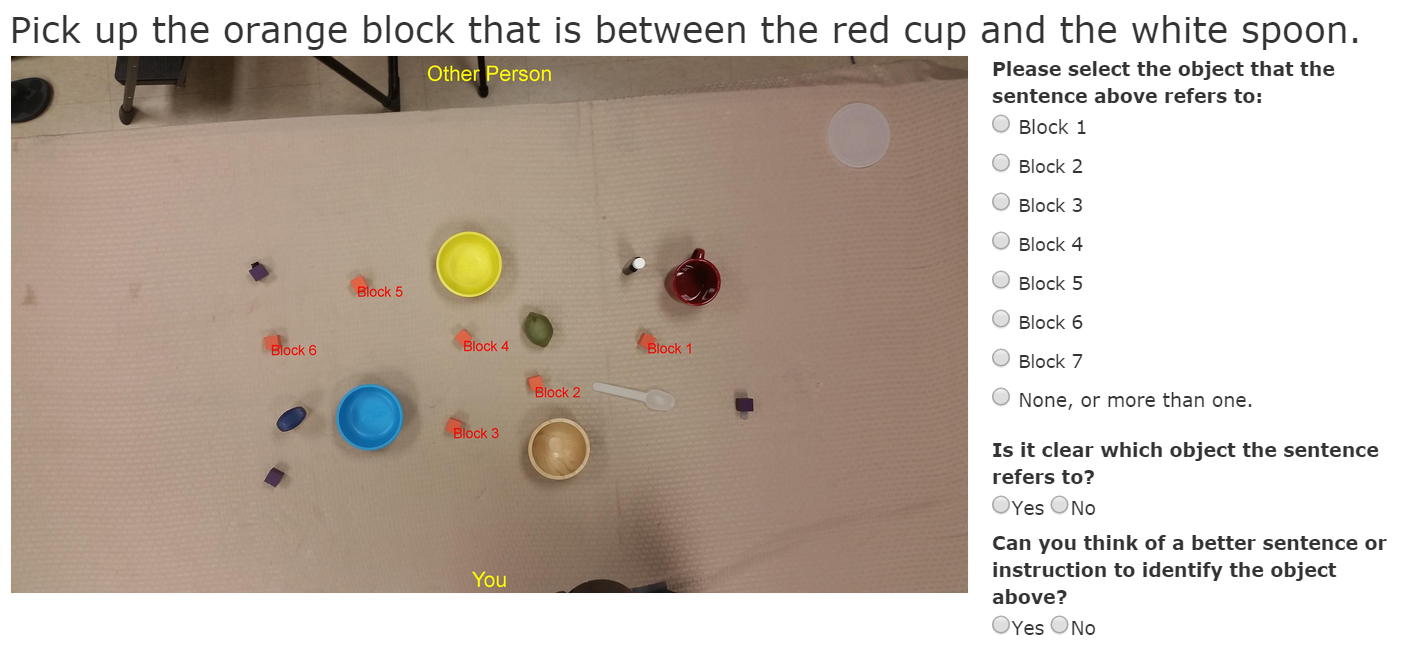
\includegraphics[width=0.90\textwidth]{ref_expr_eval_pic}}
  \caption{Example picture provided to HIT workers to evaluate referring expressions.}
  \label{fig:ref_expr_eval_pic}
\end{figure}

\subsection{Data Gathered}

\begin{figure}[h!tb]
  \centering
    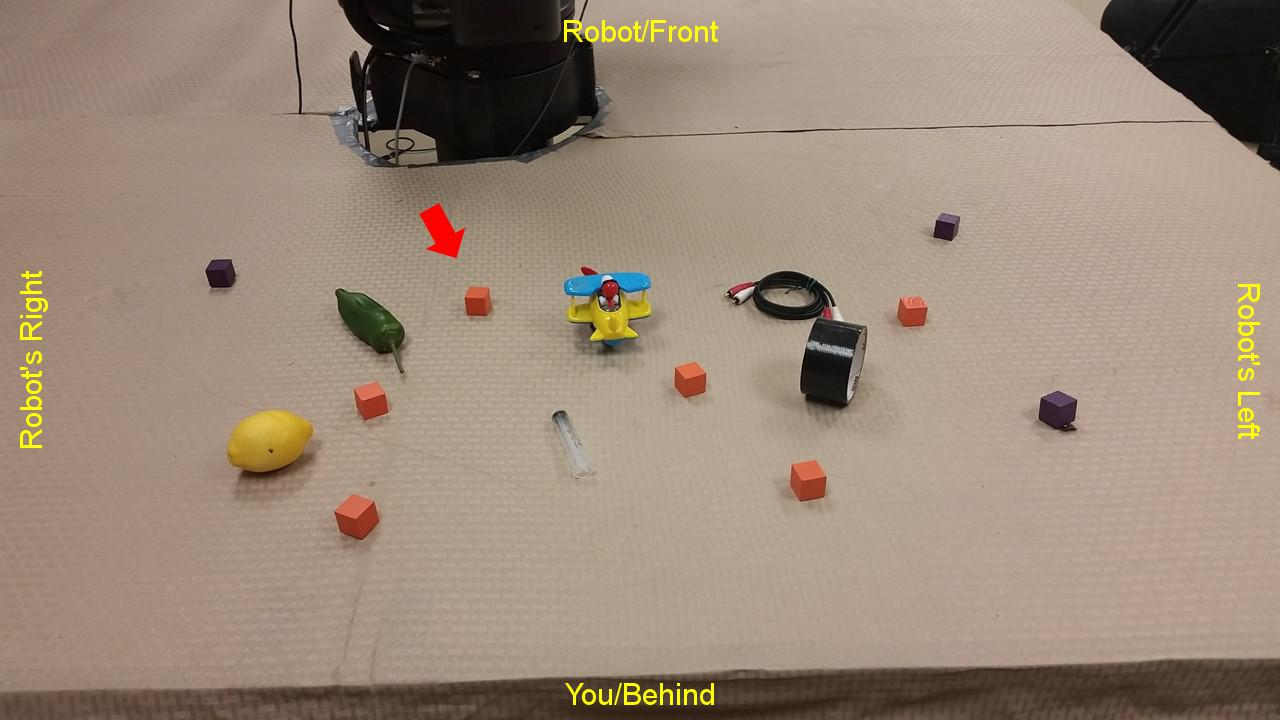
\includegraphics[width=0.75\textwidth]{ref_expr_examples_pic}
  \caption{Example picture provided to HIT workers to elicit referring expressions.}
  \label{fig:ref_expr_examples_pic}
\end{figure}

We used Figure~\ref{fig:ref_expr_examples_pic} to elicit referring expressions. Some referring expressions we received are:

\begin{itemize}[topsep=0pt,itemsep=-1ex,partopsep=1ex,parsep=1ex]
	\item I want the orange cube in front of you, between the chili and the toy.
	\item hand me the orange cube that is in between jalape\~{n}o and airplane
	\item Directly in front of you next to the green pepper and airplane.
	\item Take the orange block between the toy airplane and green chili pepper
	\item bring the orange cube between the pepper and the plane.
\end{itemize}

\section{Current Results}

We have an initial version of the algorithm which operates in batch mode. This, when run against a small test set, yields the results presented here.

\begin{figure}[H]
  \centering
  \begin{tabular}{| r r | c | c | c || c c |} \hline
     & & \multicolumn{5}{c|}{Rate of correct identification, Test (\%)} \\
     & & \multicolumn{3}{c||}{Baselines} & \multicolumn{2}{c|}{Results} \\
     \multicolumn{2}{|c|}{Preposition}
			                      &   Human & Unigram & Random &  Top-1 & Top-3 \\\hline
26.8\% & \textit{between}       & 89.8  & 0.0   & 7.1   & 71.6  & 94.1 \\
21.3\% & \textit{near}          & 76.2  & 0.0   & 7.3   & 11.1  & 54.3 \\
14.2\% & \textit{behind}        & 68.9  & 0.0   & 6.9   & 25.9  & 75.9 \\
11.0\% & \textit{in front of}   & 58.3  & 0.0   & 7.5   & 21.4  & 64.3 \\
9.4\% & \textit{left of}        & 81.5  & 0.0   & 7.3   & 25.0  & 83.3 \\
5.8\% & \textit{right of}       & 61.9  & 0.0   & 7.3   & 36.4  & 59.1 \\\hline\hline
    \multicolumn{2}{|r|}{Total} & 76.7  & 0.0   & 7.2   & 48.3  & 79.5 \\\hline
  \end{tabular}
  \caption{Performance on test set.}
  \label{fig:results}
\end{figure}

Figure~\ref{fig:results} shows the correctness rate of our algorithm and of four baselines for comparison, when run on a reduced test set. The percentage next to each preposition is the fraction of sentences in the test set that contain this preposition, and so will not add up to 100\%. The baselines are:
\begin{enumerate}[topsep=0pt,itemsep=-1ex,partopsep=1ex,parsep=1ex]
	\item The \emph{Human} baseline was established by having humans select the object best identified by the referring expression, and scoring them against our corpus.
	\item The \emph{Unigram} baseline is the expectation of selecting the correct object using a simple unigram object model across the entire input sentence.
	\item The \emph{Random} baseline is the expectation of selecting the correct object by selecting one object uniformly at random.
\end{enumerate}

The \emph{Complete} column lists the rate of correct identification using the entire sentence as input, and the \emph{SNP-1} column lists the rate using only the first simple noun phrase. It represents the success rate without using our model.

(For evaluation, the rate of correct identification is the number of trials in which the algorithm assigns a higher probability to the correct item than to any other item. The percentage on the left of each preposition is the fraction of the test set that the preposition makes up.)

To evaluate incremental performance, we will be reporting the performance on the test set as a fraction of each sentence provided to the algorithm.

\subsection{Incremental Performance}



\subsection{Future Work}
This work still remains:
\begin{enumerate}[topsep=0pt,itemsep=-1ex,partopsep=1ex,parsep=1ex]
\item Completing evaluation on a test set.
\item Incremental parsing, which requires either:
\begin{enumerate}[topsep=0pt,itemsep=-1ex,partopsep=1ex,parsep=1ex]
\item adapting the current chunker/parser for incremental work, or
\item writing a new chunker/parser entirely.
\end{enumerate}
\item Running tests on a full test set.
\item Collecting incremental user performance.
\item Writing a paper.
\end{enumerate}


\section{Related Work}

Prepositional phrases have not been subject to as much computational analysis and study as noun- and verb-phrases. However, there are still a number of papers related to the topic. 

\citet{tellex2011understanding}, \citet{UW_RSE_ICML2012}, and \citet{artzi2013weakly} all present modern models to process referring expressions.

\citet{tellex2011understanding} presents the $G^3$ framework. We use several key ideas from this paper, in particular we implicitly assume the binary correspondence variable that Tellex~et.~al. maximize the distribution of. Our algorithm is inspired in part by the algorithm they present.

\citet{UW_RSE_ICML2012} presents a state-of-the-art process to learn a models for a semantic parser and word-classifier alignment. Our approach is substantially different from Matuszek~et.~al. since we do not separate perceptual features from the language model of each object. (i.e. we do not use any visual input.) Also, in the learning phase of their algorithm, Matuszek~et.~al. calculate the marginal probability of a particular grounding and a particular word by performing a beam search over all possible parses. We assume instead that each node in the parse is independent of its sibling nodes, which allows us to use dynamic programming to incrementally build the distribution.

\citet{artzi2013weakly} trains Combinatory Categorial Grammars (CCG) with ambiguous validation functions to parse instructions, including spatial relations. While this approach is more flexible and likely performs better on entirely novel sentences, we (as we did with Matuszek~et.~al.) deliberately choose a simpler model that lends itself to a dynamic programming approach.


In addition to these, we rely on previous work about prepositional phrases:

\citet{collins95} present a model for disambiguating prepositional phrase attachments. They deal with Noun-Phrases and Verb-Phrases, but their statistical technique may be useful. This concept is also explored by \citet{ratna98}, and \citet{brill94}, each of whom suggest alternative models. Additionally, \citet{merlo97} explore disambiguating multiple prepositional phrases, rather than a single phrase between multiple targets, both of which are relevant to future work. However, our current model uses sentences focused around a single noun phrase, unlike the general English corpus used in this paper. Additionally, the incremental nature of our parsing requires an alternative framework, and as such not all techniques suggested in these papers can be used.

Another issue we face is the challenge of identifying objects and mapping them to probability distributions via language model. To deal with this, \citet{barbu13} present a model for mapping language to object models in video data and \citet{UW_RSE_ICML2012} describe an approach to the problem of simultaneously observing and extracting representations of a perceived world. These approaches can be adapted to help design features, choose objects, and select language models for prepositional phrase training, rather than using pre-defined objects and locations as we currently do, similar to the work of \citet{tellex2011understanding} which presents a method to dynamically generate a probabilistic model of a natural language input and perform inferences relating to semantic meaning. This is similar to the work we will preform in semantic parsing, though we will do so incrementally rather than with an entire sentence and thus our work will need to modify these models.

There are still a number of improvements to be made to our machine learning techniques. \citet{rudzicz03} give us a framework for parsing and understanding prepositional phrases. Similarly, \citet{liang2013learning} describe a method to create a semantic parser using question-answer pairs as data, rather than requiring annotated sentences, solving the same issue we approach of transforming natural language into semantic meaning. However, while these may be useful for generating a semantic model over entire sentences our technique will be different as we are currently only working with noun phrases, and apply additional information from the spatial model. 

\section{Conclusion}
This proposal is for an incremental referring expression parser that can process prepositional phrases. The incremental nature of the parser is the key contribution: the state-of-the-art parsers all operate on complete referring expressions. The incremental nature of this parser allows for social feedback and lower-latency interpretations of referring expressions.

\clearpage
\printbibliography

\end{document}

